% !TeX TXS-program:compile = txs:///pdflatex/[--shell-escape]
\documentclass[landscape,a4paper]{article}
\usepackage[table]{xcolor}
\usepackage[normalem]{ulem}
\usepackage{tikz}
\usetikzlibrary{shapes,positioning,arrows,fit,calc,graphs,graphs.standard}
\usepackage[nosf]{kpfonts}
\usepackage[t1]{sourcesanspro}
\usepackage{multicol}
\usepackage{wrapfig}
\usepackage[top=0.5mm,bottom=1mm,left=1mm,right=1mm]{geometry}
\usepackage[framemethod=tikz]{mdframed}
\usepackage{microtype}
\usepackage{tabularx}
\usepackage{hhline}
\usepackage{makecell}
\usepackage{mathtools}
\usepackage{subfig}
\usepackage{listings}
\usepackage{soul}
\usepackage{amsmath,amsthm,amsfonts,amssymb}
\usepackage{minted}

\graphicspath{ {./imgs/} }

\DeclarePairedDelimiter{\ceil}{\lceil}{\rceil}

\definecolor{myblue}{cmyk}{1,.72,0,.38}

\pgfdeclarelayer{background}
\pgfsetlayers{background,main}

\renewcommand{\baselinestretch}{.8}
\pagestyle{empty}

\let\counterwithout\relax
\let\counterwithin\relax
\usepackage{chngcntr}
\usepackage{verbatim}
\usepackage{etoolbox}
\makeatletter
\preto{\@verbatim}{\topsep=0pt \partopsep=0pt }
\makeatother

\counterwithin*{equation}{section}
\counterwithin*{equation}{subsection}
\usepackage{enumitem}
\newlist{legal}{enumerate}{10}
\setlist[legal]{label*=\arabic*.,leftmargin=3mm}
\setlist[itemize]{leftmargin=3mm}
\setlist[enumerate, 1]{leftmargin=3.5mm}
\setlist{nosep}

\newenvironment{descitemize} % a mixture of description and itemize
{\begin{description}[leftmargin=*,before=\let\makelabel\descitemlabel]}
	{\end{description}}
\newcommand{\descitemlabel}[1]{%
	\textbullet\ \textbf{#1}%
}
\makeatletter

\renewcommand{\section}{\@startsection{section}{1}{0mm}%
	{.2ex}%
	{.2ex}%x
	{\color{myblue}\sffamily\scriptsize\bfseries}}
\renewcommand{\subsection}{\@startsection{subsection}{1}{0mm}%
	{.2ex}%
	{.2ex}%x
	{\sffamily\bfseries}}
\renewcommand{\subsubsection}{\@startsection{subsubsection}{1}{0mm}%
	{.2ex}%
	{.2ex}%x
	{\rmfamily\bfseries}}

\makeatother
\setlength{\parindent}{0pt}
% Remove belowskip of
\setlength\partopsep{-\topsep}

\newcolumntype{a}{>{\hsize=1.5\hsize}X}
\newcolumntype{b}{>{\hsize=.25\hsize}X}

\setlength\columnsep{10pt}
\setlength\columnseprule{0pt}
\begin{document}
	\abovedisplayskip=0pt
	\abovedisplayshortskip=0pt
	\belowdisplayskip=0pt
	\belowdisplayshortskip=0pt
	\scriptsize
%	\tiny
	\begin{multicols*}{4}
		\section{Introduction}
		\subsection{Types of Analysis}
		\begin{itemize}
			\item \textbf{Descriptive Analytics}: What happened? What is happening?
			\item \textbf{Predictive Analytics}: What will happen?
			\item \textbf{Prescriptive Analytics}: What to do?
		\end{itemize}
		\section{R Basics}
		\subsection{Working Environment}
		\begin{itemize}
			\item \textbf{Workspace}: contains all variables and functions (collectively known as \textbf{objects}) as well as any packages loaded
			\item \textbf{Working directory}: Default directory where R will look for files loaded/stored
			\item \textbf{Project}: Data, R scripts, analytical results, and figures about a particular problem are normally organised and stored under one project
		\end{itemize}
		\subsubsection{Relavent Commands}
		\begin{itemize}
			\item \mintinline{r}|getcwd()|: get working directory
			\item \mintinline{r}|setwd(<dir>)|: sets the working directory to <dir>
			\item \mintinline{r}|ls()|: lists all objects (variables and functions) defined in the current work space
			\begin{itemize}
				\item We can use \mintinline{r}|rm(<obj>)| to remove
			\end{itemize}
			\item \mintinline{r}|dir()|: lists all files and subfolders in cwd
			\begin{itemize}
				\item \mintinline{r}|list.files()| does the same as \mintinline{r}|dir()|
			\end{itemize}
			\item \mintinline{r}|file.exists(<file>)|: checks if a certain file exist
			\begin{itemize}
				\item Useful when we want to check if dir exists before creating it
				\item \mintinline{r}|ifelse(!dir.exists("a"),dir.create("a"),"a exists")|
			\end{itemize}
		\end{itemize}
		\subsection{Atomic Data Types}
		R has 5 basic (atomic) data types
		\begin{itemize}
			\item \textbf{Logical}
			\begin{itemize}
				\item TRUE or FALSE, T or F
				\item In terminal output, will always be TRUE/FALSE
				\item Return value of logical operators: <, >, |, \&, !
			\end{itemize}
			\item \textbf{Numeric}
			\begin{itemize}
				\item Decimal values, e.g. 1.23
				\item \textcolor{red}{By default, if we assign integer to variable, the class will be numeric, e.g. \mintinline{r}|k<-2|, $k$ will be numeric}
				\item We cannot cast strings to integer or numeric, will have warning of \texttt{NAs introduced by coercion}
			\end{itemize}
			\item \textbf{Integer}
			\begin{itemize}
				\item To convert numeric to integer, have to use the \mintinline{r}|as.integer(<num>)| function
				\item Note that the \mintinline{r}|as.integer(<num>)| will always round down, i.e. 2.34 $\rightarrow$ 2 and 2.56 $\rightarrow$ 2
			\end{itemize}
			\item \textbf{Character}
			\begin{itemize}
				\item Basically string data type in R
				\item Can use \mintinline{r}|nchar(<string>)| to find number of characters
				\item To find index of matches within a string \mintinline{r}|regexpr(<pattern>, <string>)|, will return -1 if no results found e.g.
				\begin{minted}{r}
regexpr("ex", "longtext")
## [1] 6
## attr(,"match.length")
## [1] 2
## attr(,"index.type")
## [1] "chars"
## attr(,"useBytes")
## [1] TRUE
				\end{minted}
				\item Can use \mintinline{r}|gregexpr(<pattern>, <string>)| to find positions of every match
				\item Can use \mintinline{r}|grep(<pattern>, <vector>)| to  find the positions of a regular expression in a vector of text strings
				\item Use \mintinline{r}|substr(<string>, <start>, <end>)| to get a slice of from start to end (inclusive). \textcolor{red}{Strings are 1-indexed}
				\item Use \mintinline{r}|sub(<pattern>, <replacement>, <string>)| to replace the first match of a string with a new string and \mintinline{r}|gsub()| to replace all matches
			\end{itemize}
		\end{itemize}
		\subsection{Data Structures}
		\subsubsection{Vectors}
		\begin{itemize}
			\item ordered array of elements of the \textcolor{red}{same data type}
			\item Created using \mintinline{r}|arr<-c(1,2,3)|
			\item \textcolor{red}{Data coercion} to most flexible data type if trying to store multiple data types
			\begin{itemize}
				\item In order of \textbf{boolean > int > numeric > character}
			\end{itemize}
			\item Can check the type of vector using \mintinline{r}|typeof()|
			\item Can name vectors using:
			\begin{minted}{r}
a<-c(1,3,4)
furniture <- c("desks", "tables", "chairs")
names(a) <- furniture

a<-c("desks" = 1, "tables" = 3, "chairs" = 4)

a<-c(desks = 1, tables = 3, chairs = 4)
			\end{minted}
		\end{itemize}
		\subsubsection{Vector Arithmetic}
		\begin{itemize}
			\item \mintinline{r}|arr + 100| will add 100 to each element in the vector
			\item Can also do the standard + - * / \^{} operations
			\item Math operations \textcolor{red}{will not work} on strings
			\item Can also do operations on 2 vectors
			\begin{itemize}
				\item \texttt{c(1,2,3,4)+c(1,2,3)->c(2,4,6,5)} + warning (\textbf{recycling})
			\end{itemize}
			\item Possible to use \texttt{mean, prod, sum} methods too
		\end{itemize}
		\subsubsection{Vector Subsetting}
		\begin{itemize}
			\item As in python, use [] to access elements in vector
			\item Can access using their indexes or their name
			\item Access multiple elements by doing \mintinline{r}|materials[c(4,3)]|
			\item Possible to use \mintinline{r}|moreMetals[-6]| which selects all other indexes besides 6th element
			\item Can also index using \mintinline{r}|arr[c(TRUE, TRUE, FLALSE)]|, if inner boolean array < size of arr, recycling will happen, if size inner array > size of arr, NA will be returned
		\end{itemize}
		\subsubsection{Matrices}
		\begin{itemize}
			\item Matrix are arranged \textbf{by default by columns}, to change it to by row, use \mintinline{r}|matrix(3:8,ncol = 3,nrow = 2,byrow = TRUE)|
			\item \textcolor{red}{Matrices are fundamentally vectors}
			\item \textcolor{red}{Can only contain homogeneous data types}
			\item To create a matrix:
			\begin{minted}{r}
matrix(3:8,ncol=3,nrow=2)

matrix(3:8,nrow=2)

m2<-3:8
dim(m2)<-c(2,3)

##      [,1] [,2]
## [1,]    3    6
## [2,]    4    7
## [3,]    5    8
			\end{minted}
			\item If nrow $\times$ ncol > range of number supplied, recycling will happen
			\begin{minted}{r}
matrix(3:5,ncol=3,nrow=2)

##      [,1] [,2] [,3]
## [1,]    3    5    4
## [2,]    4    3    5
			\end{minted}
			\item If length of input arr not a multiple of nrow $\times$ ncol, warning will be thrown
			\item Can name columns and rows using
			\begin{minted}{r}
rownames(m3)<-c("Row1","Row2")
colnames(m3)<-c("Col.1","Col.2","Col.3")
			\end{minted}
			\item Matrix access is by [row, col]
		\end{itemize}
		\subsubsection{Factors}
		\begin{itemize}
			\item Factors are special variables used to store \textbf{categorical variables}
			\item Advantages of using factors:
			\begin{itemize}
				\item Factor variables are stored as a vector of integer values, thus it is a more efficient use of memory
				\item statistical models will automatically handle factor variables properly
				\item useful in graphics
			\end{itemize}
			\item To create factors:
			\begin{minted}{r}
a<-c(0,1,0,0,1)
a.f<-factor(a,labels = c("Male","Female"))

a<-c("One","Two","Three","One","Three")
a.f<-factor(a)
			\end{minted}
			\item Levels in factors are \textbf{ordered in lexicographical order}, have to manually assign them to avoid this
		\end{itemize}
		\subsubsection{List}
		\begin{itemize}
			\item Allows for multiple types to be stored in the same array
			\item Created using:
			\begin{minted}{r}
list(Name="Mike",Age=43,Children=c("Tom","Lily"))
			\end{minted}
			\item Can access elements using the standard [] operator or using the \$ symbol, e.g. \mintinline{r}|lst$Age|
			\item Use the \texttt{str} command to display the internal structure of a list
			\begin{minted}{r}
str(Mike)

## List of 4
##  $ Name    : chr "Mike"
##  $ Salary  : num 10000
##  $ Age     : num 43
##  $ Children: chr [1:3] "Tom" "Lily" "Alice"
			\end{minted}
		\end{itemize}
		\columnbreak
		\subsubsection{DataFrames}
		\begin{itemize}
			\item Basically a matrix that can contain heterogeneous data types
			\item Is just a \textcolor{red}{list of vectors}, can use \texttt{length} to get the number of rows
			\item Created using the \mintinline{r}|data.frame()| method
			\begin{minted}{r}
name <- c("Anne", "Pete", "Frank", "Julia", "Cath")
age <- c(28, 30, 21 ,39, 35)
child <- c(FALSE, TRUE, TRUE, FALSE, TRUE)

df <- data.frame(name, age, child)
			\end{minted}
			\item Can also name the cols using \mintinline{r}|names(<df>)| function
			\item \textcolor{red}{Will automatically convert character data type into factors}
			\begin{itemize}
				\item If we want to store them as characters, use \mintinline{r}|data.frame(name, age, child, stringsAsFactors=FALSE)|
			\end{itemize}
			\item Subsetting is the same as in matrices, the following results are returned as a \textbf{Dataframe}
			\begin{minted}{r}
df[3,2] ## Select element in row 3, col 2
df[3,"age"] ## Select row 3, with col name of "age"
df[3,] ## select entire row 3
df[,"age"] ## select entire col with name "age"
df[c(3,5), c("age", "child")]
			\end{minted}
			\item If we want to return them as a \textbf{list}
			\begin{minted}{r}
df$age
df[["age"]]
df[[2]]
			\end{minted}
			\item We can extend dataframes using \mintinline{r}|cbind()| or \mintinline{r}|rbind()|
			\item Sorting dataframes
			\begin{itemize}
				\item \mintinline{r}|sort(df$age)| return ascending order of "age" column
				\item \mintinline{r}|order(df$age)| return order of the current indexes if sorted
				\item \mintinline{r}|max(df$age)| returns max \textbf{value} of "age" column
				\item \mintinline{r}|which.max(df$age)| return \textbf{index} of element with max value in "age" column
				\item \mintinline{r}|rank(df$age)| return current ranking of each element
			\end{itemize}
			\item Indexing dataframe
			\begin{itemize}
				\item \mintinline{r}|df[df$age > 30 & df$child == FALSE,]|
				\item \mintinline{r}|which(df$name == "Cath")| returns index where name == "Cath"
				\item \mintinline{r}|match(c("Anne", "Julia", "Cath"), df$name)| return indexes that match those names
				\mintinline{r}|c("Anne", "Julia", "Cath", "Bob") %in% df$name|
			\end{itemize}
		\end{itemize}
		\section{Data Wrangling}
		\subsection{Built-in}
		\begin{itemize}
			\item \mintinline{r}|read.csv(<file>)| to read CSV files
			\item \mintinline{r}|read.csv2(<file>)| to read semicolon seperated file
			\item \mintinline{r}|read.delim(<file>)| to specify the delimeter
			\item \mintinline{r}|summary(<matrix>)| returns min, 1st quartile, median, mean, 3rd quartile, max and number of NAs for each col
		\end{itemize}
		\subsection{Dplyr}
		\begin{itemize}
			\item \mintinline{r}|mutate(df, bmi = weight/height^2*10000)| add a new col bmi
			\item \mintinline{r}|filter(df, bmi > 18.5 & bmi < 24.9)| filters out rows that match the condition
			\item \mintinline{r}|select(df, name, height)| select name and heigh col of df
			\item \mintinline{r}|intersect(<arr>, <arr>)| returns common element between 2 vectors/dataframe
			\item \mintinline{r}|union(<arr>, <arr>)| returns the union of the 2 vectors/dataframes, taking into account of duplicates
			\item \mintinline{r}|setdiff(<arr>, <arr>)|, usage:
			\begin{minted}{r}
setdiff(1:10, 6:15) ## [1] 1 2 3 4 5
setdiff(6:15, 1:10) ## [1] 11 12 13 14 15
			\end{minted}
			\item \mintinline{r}|setequal(<arr>, <arr>)| returns whether 2 sets/dataframes are same, \textcolor{red}{regardless of order}
		\end{itemize}
		\subsection{readr}
		\begin{center}
			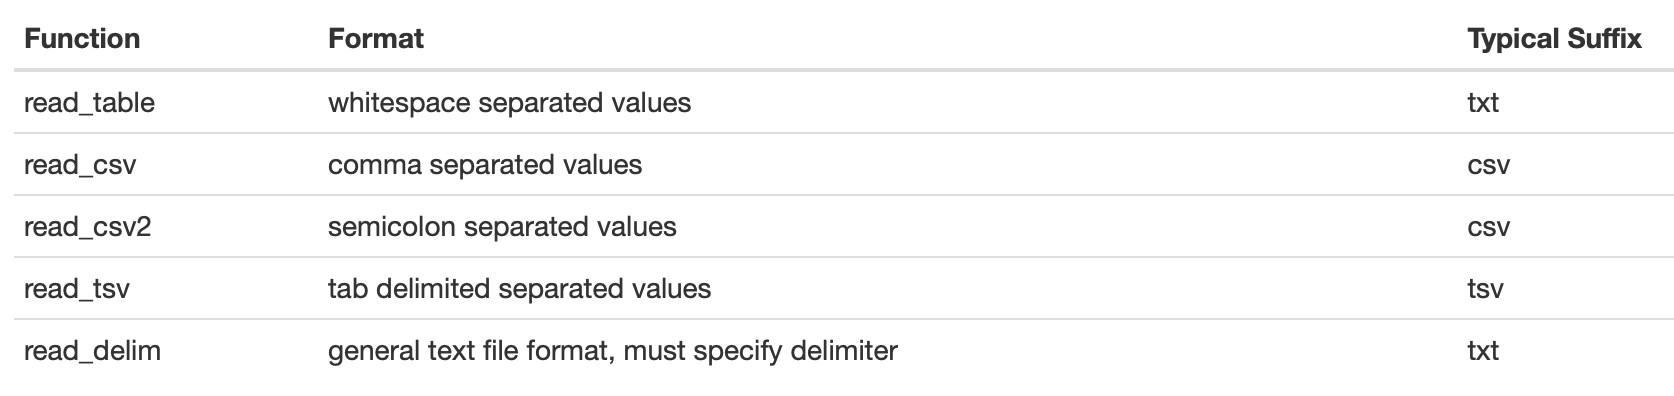
\includegraphics[width=0.95\columnwidth]{readr}
		\end{center}
		\subsection{readxl}
		\begin{center}
			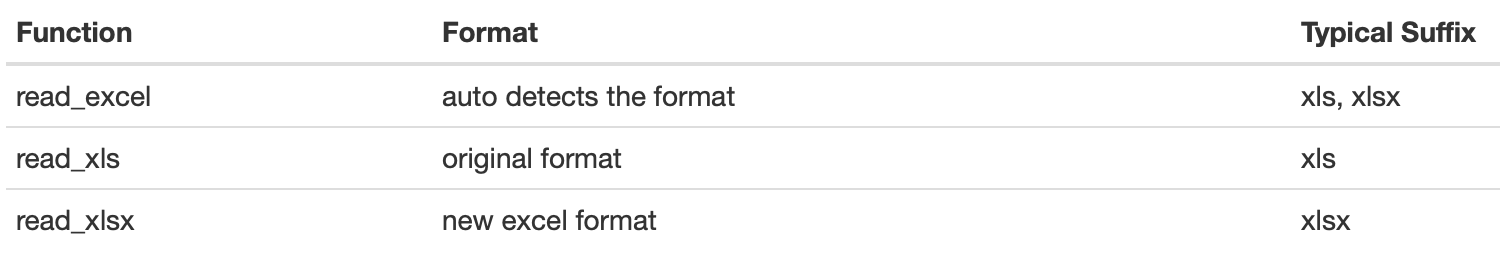
\includegraphics[width=0.95\columnwidth]{readxl}
		\end{center}
		\subsection{jsonlite}
		\begin{minted}{r}
url <- "https://api.data.gov.sg/v1/carpark-availability"
data <- fromJSON(url)
a <- as.data.frame(data$items$carpark_data)
		\end{minted}
		\subsection{XML}
		\begin{minted}{r}
data <- xmlParse("books.xml")
root <- xmlRoot(data) # get root node
nodes <- xmlChildren(root) # get child nodes of root
a <- nodes[[2]] # get 2nd child of root
books <- getNodeSet(data, "/catalog/book[@type='HardCover']")
xmlToList(date)
xmlToDataFram(books)
		\end{minted}
		\subsection{tidyr}
		\begin{center}
			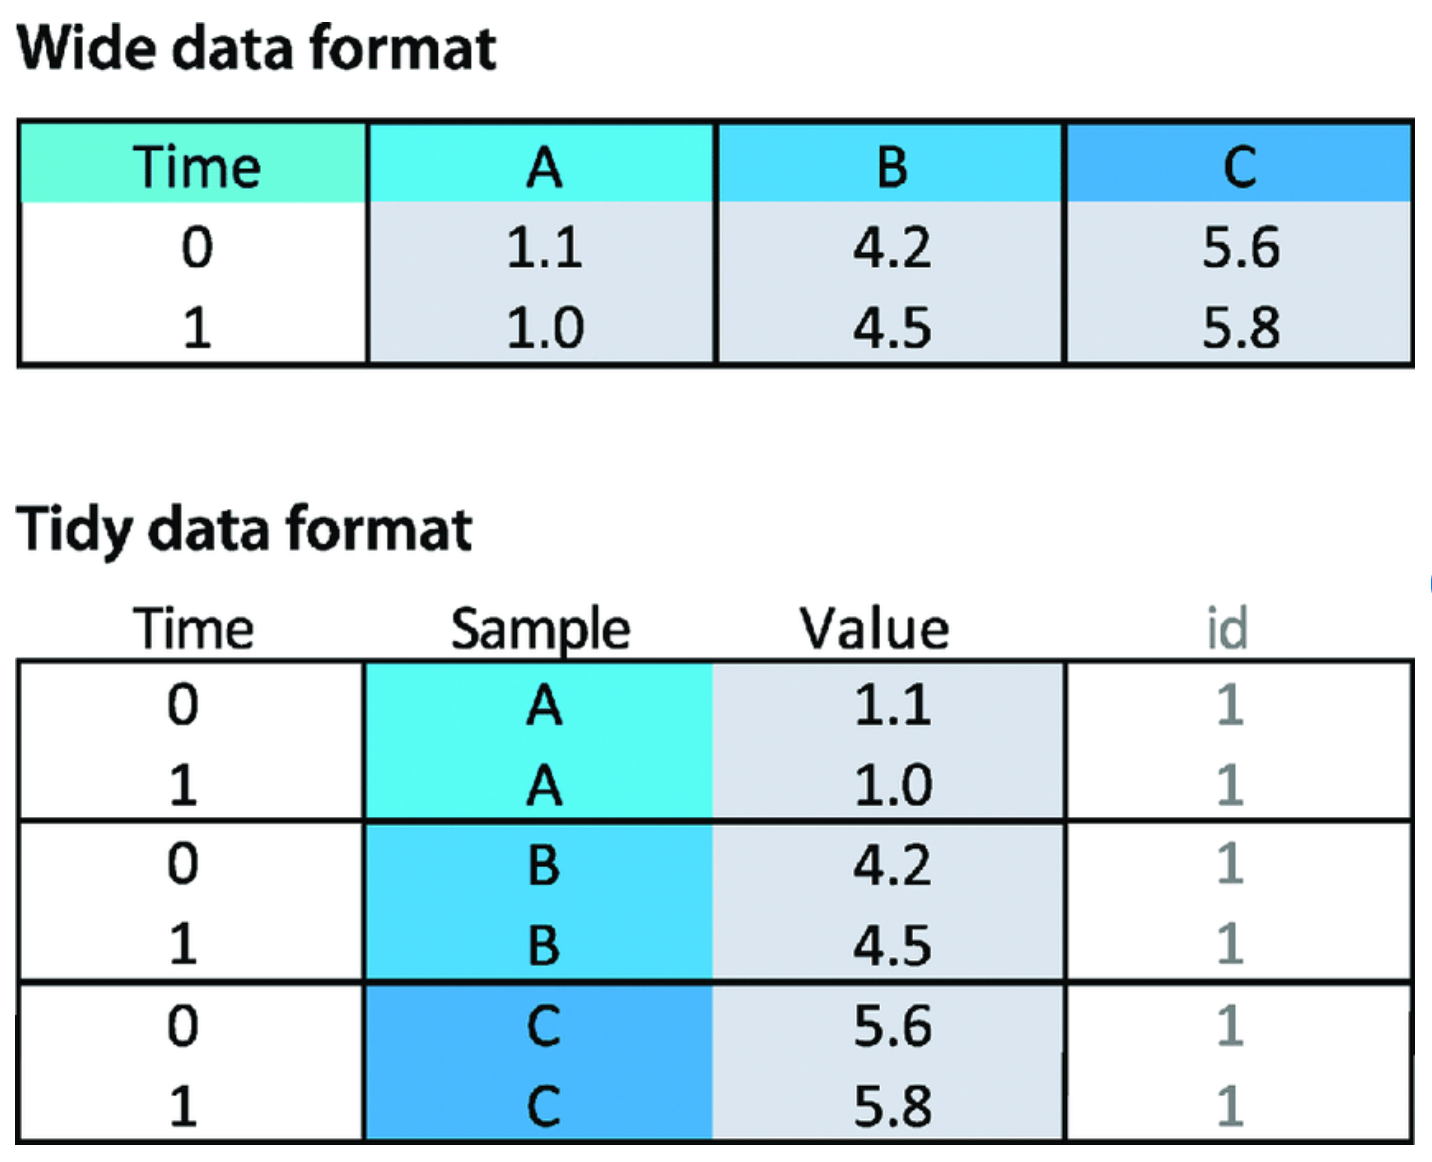
\includegraphics[width=0.7\columnwidth]{tidy-vs-wide}
		\end{center}
		\begin{itemize}
			\item Main use is to reshape data, from wide to tidy
			\item \mintinline{r}|wide_data %>% gather(year, fertility, '1960':'2015')|
			\begin{itemize}
				\item first argument will be the name of column for the gathered variables
				\item second argument is for the values in the column cells
				\item third argument in the function to specify the specific columns to gather
			\end{itemize}
			\item Can change from tidy to wide using \mintinline{r}|spread()| command
		\end{itemize}
		\subsection{Joins}
		\begin{itemize}
			\item \mintinline{r}|left_join(<table>, <table>, by=c('col'='col'))| join right into left with matching entries, keep everything in left
			\item \mintinline{r}|right_join(<table>, <table>, by=c('col'='col'))| join left into right with matching entries, keep everything in right
			\item \mintinline{r}|inner_join(<table>, <table>, by=c('col'='col'))| basically intersection of 2 tables
			\item \mintinline{r}|full_join(<table>, <table>, by=c('col'='col'))| basically a union of 2 tables
			\item \mintinline{r}|semi_join(<table>, <table>, by=c('col'='col'))| allows us to keep the part of the first table for which we have information in the second table, but doesnt add the columns of the second
			\item \mintinline{r}|anti_join(<table>, <table>, by=c('col'='col'))| allows us to keep the part of the first table for which we have NO information in the second table, but doesnt add the columns of the second
		\end{itemize}
		\section{Programming Structure and Functions}
		\begin{enumerate}
			\item Conditionals
			\begin{minted}{r}
if(boolean condition){
    expressions
} else{
    alternative expressions
}

ifelse(boolean condition,expressions,alt expressions)
			\end{minted}
			\item \mint{r}|any(<vector>)| returns TRUE if any of logicals are true
            \item \mint{r}|all(<vector>)| returns TRUE if all of logicals are true
            \item Functions
            \begin{minted}{r}
my_function <- function(x, y, z=1){
    operations that operate on x, y, z
    value of final line is returned
}
            \end{minted}
            \item For loops
            \begin{minted}{r}
for (i in range of values){
    operations that use i
}
            \end{minted}
            \item \mint{r}|apply(x, MARGIN, FUNC, <args>)| applies FUNC over each element of a matrix/dataframe. Margin=1 will apply row wise, Margin=2 will apply col wise
		\end{enumerate}
	\end{multicols*}
\end{document}